\newpage
\subsection*{Single Side Band -- Suppressed Carrier (SSB-SC)}
\addcontentsline{toc}{subsection}{SSB-SC}
The SSB-SC signal is implemented by first generating a DSB-SC signal and then eliminating
one of the sidebands using frequency-domain processing. In the implementation, the message
signal is modulated with the carrier to produce a DSB-SC signal, after which either the
upper or lower sideband is retained while the other is suppressed. Time-domain plots are
used to observe the modulated waveform, and frequency-domain analysis is performed to
confirm the presence of only a single sideband with the carrier fully suppressed.

\subsubsection*{Code (Filter Method):}

\begin{minted}[linenos, fontsize=\small]{python}
import numpy as np
import matplotlib.pyplot as plt
from scipy.signal import butter, filtfilt

# Sampling parameters
Fs = 10000               # Sampling frequency (Hz)
T = 0.1                  # Duration of signal (seconds)
t = np.arange(0, T, 1/Fs)

# Message signal
Am = 1
fm = 50
m_t = Am * np.sin(2 * np.pi * fm * t)

# Carrier signal
Ac = 1
fc = 1000
c_t = Ac * np.cos(2 * np.pi * fc * t)

# Generate DSB-SC signal
s_dsbsc = m_t * c_t  # Suppressed carrier

# Design band-pass filter to select upper sideband (USB)
lowcut = fc           # Hz
highcut = fc + 2*fm   # Hz

# Butterworth bandpass filter
order = 6
b, a = butter(order, [lowcut/(Fs/2), highcut/(Fs/2)], btype='band')
s_usb = filtfilt(b, a, s_dsbsc)

# Plot time-domain signals
plt.figure(figsize=(12,8))

plt.subplot(3,1,1)
plt.plot(t, m_t, 'b', linewidth=1.5)
plt.title('Message Signal m(t)')
plt.xlabel('Time [s]')
plt.ylabel('Amplitude')
plt.grid(True)

plt.subplot(3,1,2)
plt.plot(t, s_dsbsc, 'g', linewidth=1.5)
plt.title('DSB-SC Signal s(t)')
plt.xlabel('Time [s]')
plt.ylabel('Amplitude')
plt.grid(True)

plt.subplot(3,1,3)
plt.plot(t, s_usb, 'r', linewidth=1.5)
plt.title('SSB-SC Signal (Upper Sideband)')
plt.xlabel('Time [s]')
plt.ylabel('Amplitude')
plt.grid(True)

plt.tight_layout()
plt.show()

# Frequency-domain analysis
N = len(s_usb)
S_f = np.fft.fft(s_usb)/N
f = np.fft.fftfreq(N, 1/Fs)
f_pos = f[:N//2]
S_f_pos = 2 * np.abs(S_f[:N//2])

plt.figure(figsize=(10,4))
plt.plot(f_pos, S_f_pos, 'm', linewidth=1.5)
plt.title("Magnitude Spectrum of SSB-SC Signal (USB)")
plt.xlabel("Frequency [Hz]")
plt.ylabel("Magnitude")
plt.grid(True)
plt.xlim(fc-50, fc+2*fm+50)  
plt.show()
\end{minted}

\subsubsection*{Output:}
The above plots are obtained using the following parameters: sampling frequency
$F_s = 10~\text{kHz}$, signal duration $T = 0.1~\text{s}$, message amplitude
$A_m = 1$, carrier amplitude $A_c = 1$, message frequency $f_m = 50~\text{Hz}$,
and carrier frequency $f_c = 1000~\text{Hz}$. Butterworth band-pass filter order = 6.

\begin{figure}[h!]
    \centering
    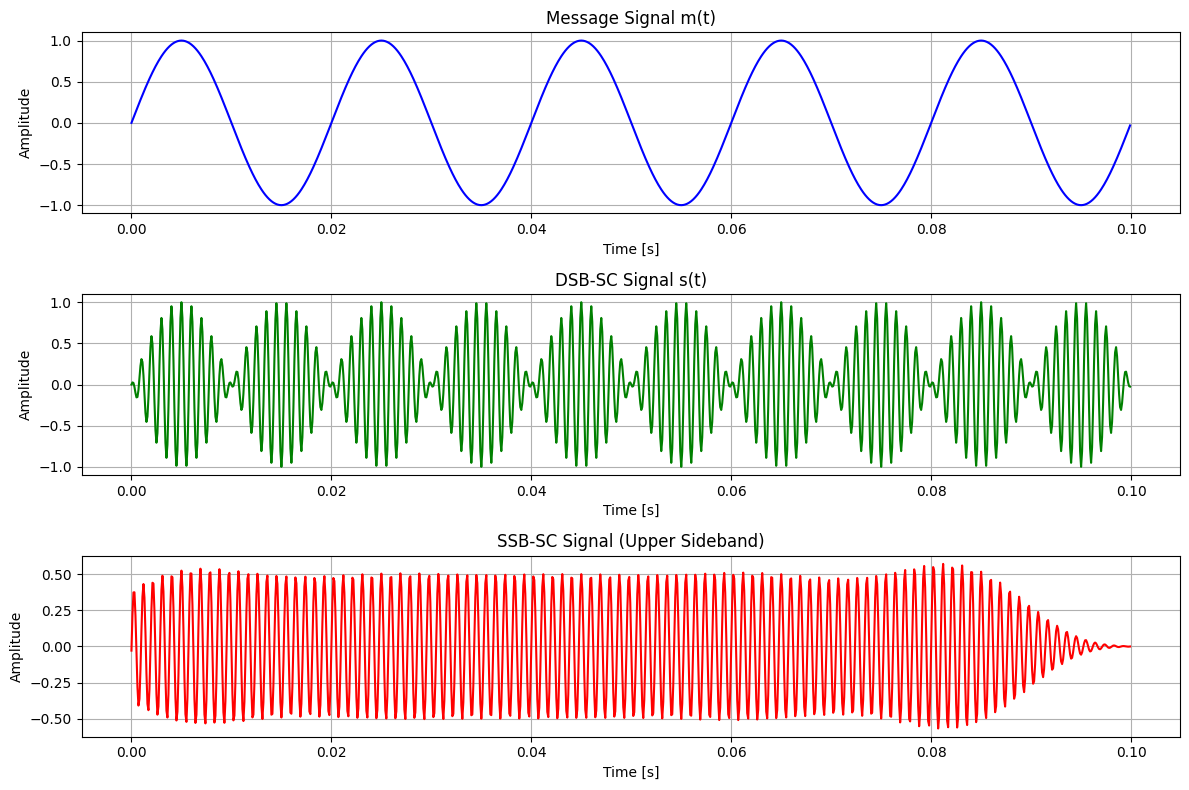
\includegraphics[width=0.9\textwidth]{images/output6.png} 
    \caption{Plots of (a) Message Signal, (b) Carrier Signal, and (c) SSB-SC Modulated Signal}
    \label{fig:output6}
\end{figure}
\begin{figure}[h!]
    \centering
    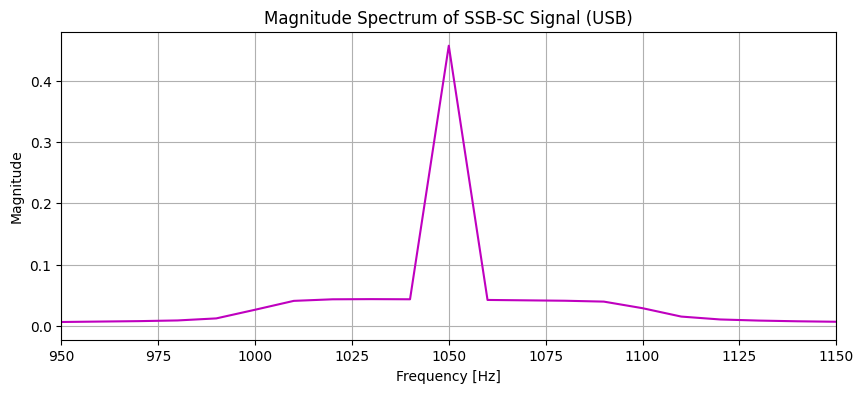
\includegraphics[width=0.9\textwidth]{images/output7.png} 
    \caption{Plots of SSB-SC spectrum}
    \label{fig:output7}
\end{figure}

\begin{figure}[h!]
    \centering
    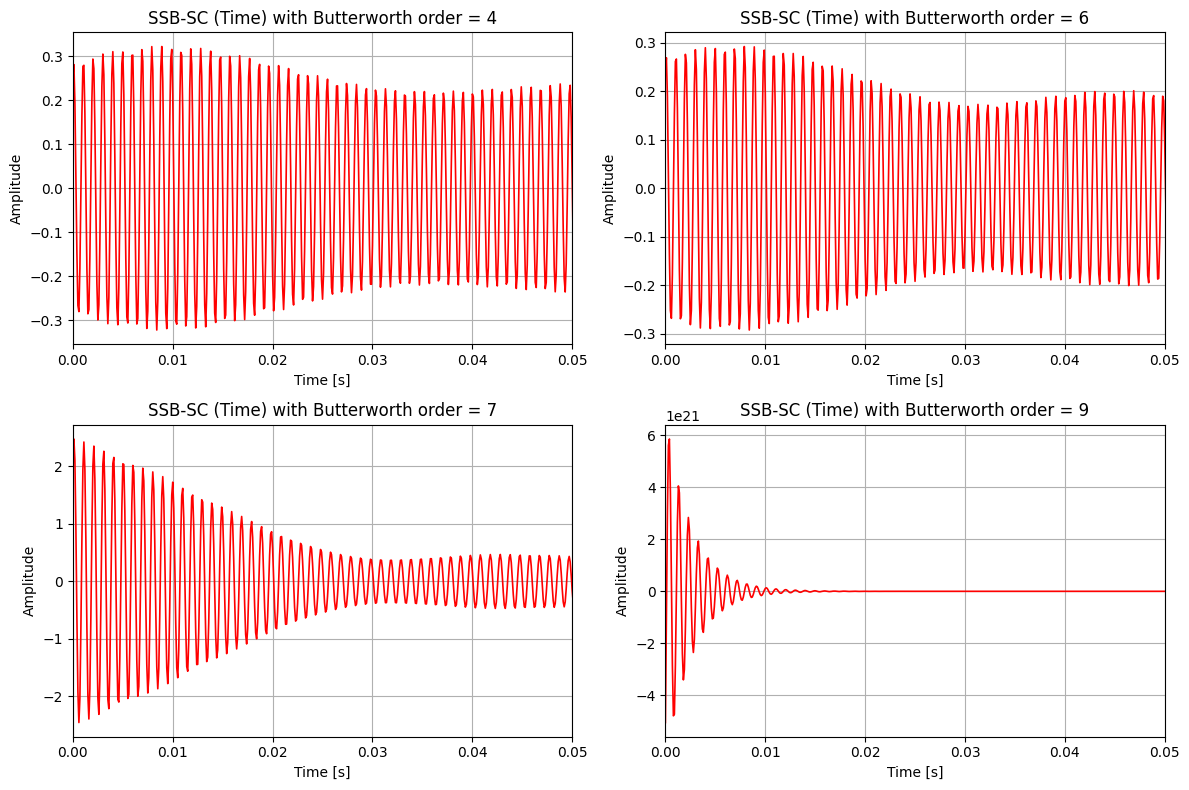
\includegraphics[width=0.9\textwidth]{images/order1.png} 
    \caption{Time-domain waveforms of SSB-SC signal for different BW filter orders}
    \label{fig:order1}
\end{figure}
\begin{figure}[h!]
    \centering
    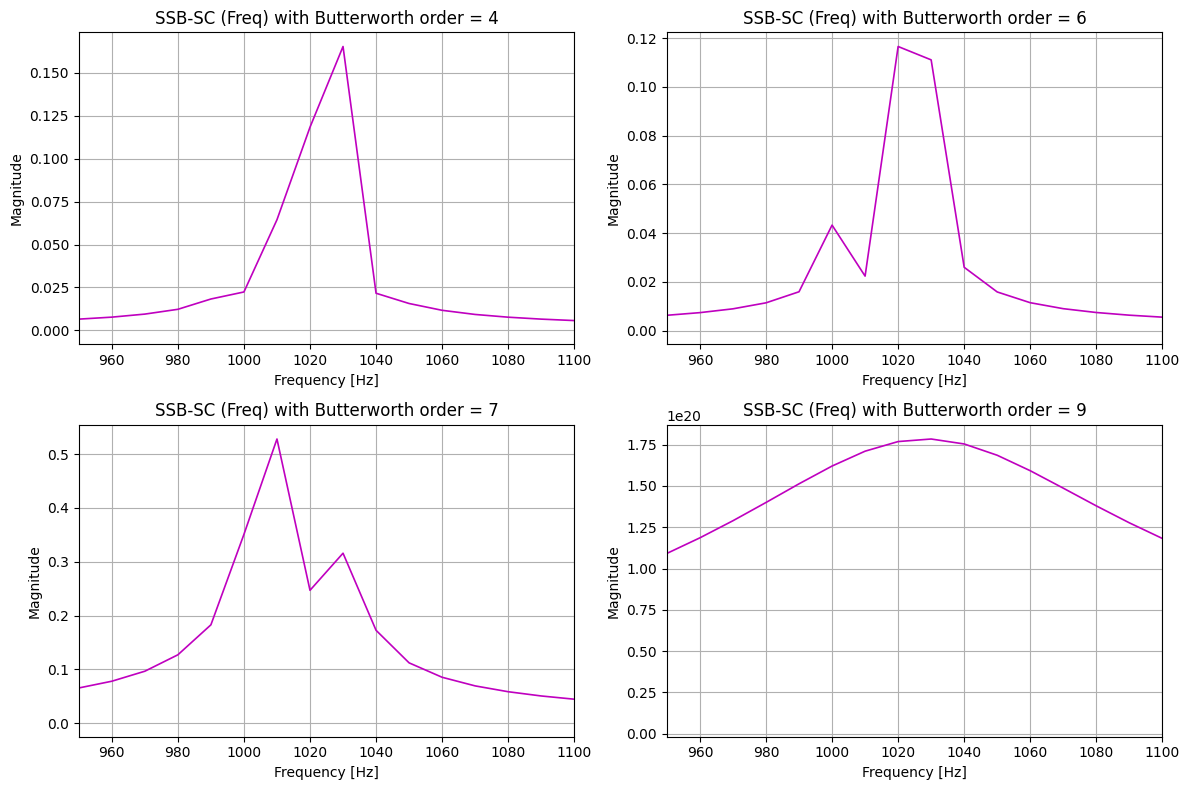
\includegraphics[width=0.9\textwidth]{images/order2.png} 
    \caption{Frequency-domain magnitude spectra of SSB-SC signal for different BW filter orders}
    \label{fig:order2}
\end{figure}

\subsubsection*{Observations:}
The DSB-SC signal contains both upper and lower sidebands, symmetric around the carrier frequency. After applying the band-pass (BW) filter, only the upper sideband is retained, while the lower sideband is suppressed, forming the SSB-SC signal. The time-domain plot of the SSB-SC signal shows a waveform with reduced amplitude oscillations compared to DSB-SC, as one sideband has been removed. The frequency-domain plot confirms that only the frequencies above the carrier (upper sideband) remain, while the carrier and lower sideband components are effectively suppressed. By Using this method, the bandwidth of the transmitted signal is halved compared to DSB-SC, which shows the bandwidth efficiency of SSB-SC.  

Increasing the BW filter order improves upper and lower sideband separation, moving the peaks closer to the true sideband frequency. Low orders allow leakage and slightly shifted peaks, while very high orders produce cleaner sidebands with minor ripple effects.


\subsubsection*{Code (Phase Discrimination Method):}
\begin{minted}[linenos, fontsize=\small]{python}
import numpy as np
import matplotlib.pyplot as plt
from scipy.signal import hilbert

# Sampling Parameters
Fs = 10000                  # Sampling frequency (Hz)
T = 0.1                     # Duration of signal (s)
t = np.arange(0, T, 1/Fs)   # Time vector

# Message Signal (Baseband)
Am = 1                      # Message amplitude
fm = 50                     # Message frequency
m_t = Am * np.sin(2 * np.pi * fm * t)  # Baseband signal

# Carrier Signal
fc = 1000                    # Carrier frequency
c_cos = np.cos(2 * np.pi * fc * t)    # In-phase carrier
c_sin = np.sin(2 * np.pi * fc * t)    # (90° phase shift)

# Hilbert Transform of Message
m_hilbert = np.imag(hilbert(m_t))

# Upper Sideband (USB)
s_usb = m_t * c_cos - m_hilbert * c_sin

# Lower Sideband (LSB)
s_lsb = m_t * c_cos + m_hilbert * c_sin

# Time-Domain Plots
plt.figure(figsize=(12, 8))

plt.subplot(3,1,1)
plt.plot(t, m_t, 'b', linewidth=1.5)
plt.title('Message Signal m(t)')
plt.xlabel('Time [s]')
plt.xlim(0, 0.05)
plt.ylabel('Amplitude')
plt.grid(True)

plt.subplot(3,1,2)
plt.plot(t, s_usb, 'r', linewidth=1.5)
plt.title('SSB-SC Signal (Upper Sideband)')
plt.xlabel('Time [s]')
plt.ylabel('Amplitude')
plt.xlim(0, 0.05)
plt.grid(True)

plt.subplot(3,1,3)
plt.plot(t, s_lsb, 'g', linewidth=1.5)
plt.title('SSB-SC Signal (Lower Sideband)')
plt.xlabel('Time [s]')
plt.xlim(0, 0.05)
plt.ylabel('Amplitude')
plt.grid(True)

plt.tight_layout()
plt.show()

# Frequency-Domain Analysis
def plot_spectrum(signal, title, Fs):
    N = len(signal)
    S_f = np.fft.fft(signal)/N
    f = np.fft.fftfreq(N, 1/Fs)
    f_pos = f[:N//2]
    S_f_pos = 2 * np.abs(S_f[:N//2])
    
    plt.figure(figsize=(10,4))
    plt.plot(f_pos, S_f_pos, 'm', linewidth=1.5)
    plt.title(title)
    plt.xlabel('Frequency [Hz]')
    plt.ylabel('Magnitude')
    plt.grid(True)
    plt.xlim(fc - 100, fc + 200)  
    plt.show()

# Plot spectra
plot_spectrum(s_usb, 'Magnitude Spectrum of SSB-SC (USB)', Fs)
plot_spectrum(s_lsb, 'Magnitude Spectrum of SSB-SC (LSB)', Fs)
\end{minted}

\newpage
\subsubsection*{Output:}
The above plots are obtained using the following parameters: sampling frequency 
$F_s = 10~\text{kHz}$, signal duration $T = 0.1~\text{s}$, message amplitude 
$A_m = 1$, carrier amplitude $A_c = 1$, message frequency $f_m = 50~\text{Hz}$, and carrier frequency $f_c = 1000~\text{Hz}$.

\vspace{5mm}

\begin{figure}[H]
    \centering
    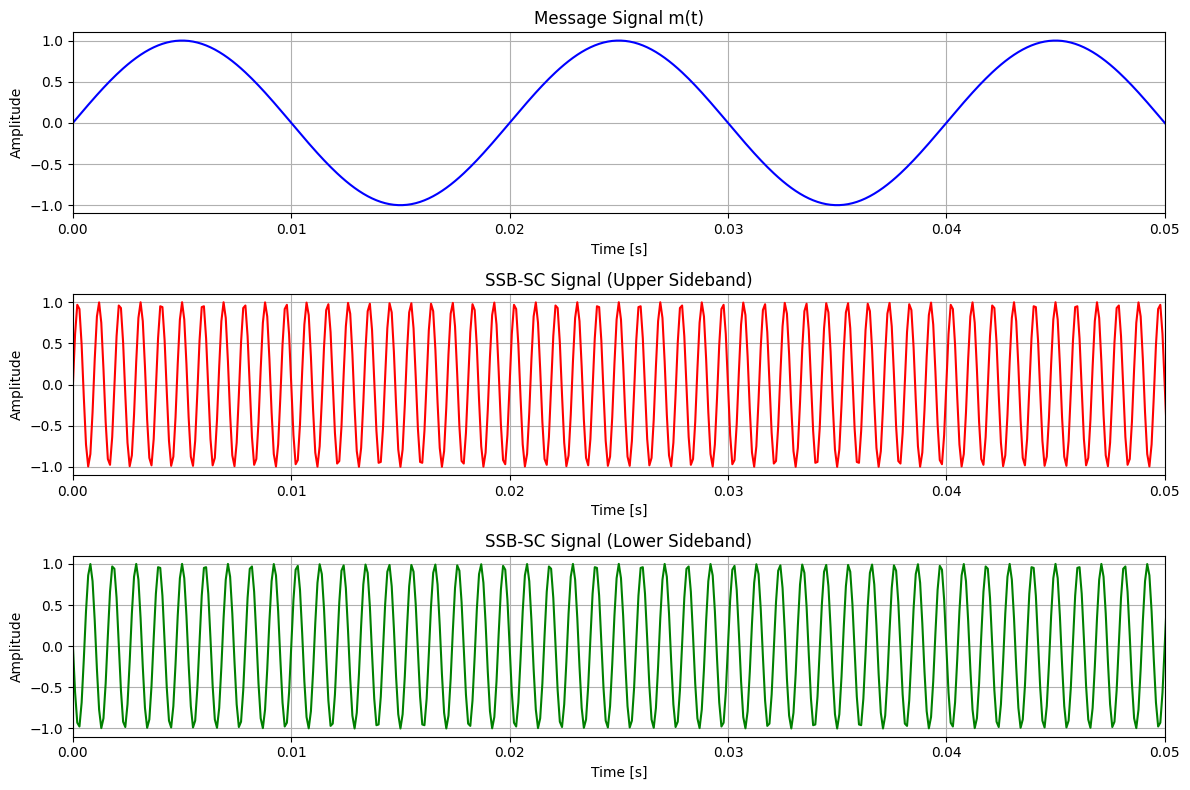
\includegraphics[width=0.9\textwidth]{images/output8.png} 
    \caption{Plots of (a) Message signal, (b) Carrier signal, and (c) SSB-SC modulated signal.}
    \label{fig:phase_output1}
\end{figure}

\begin{figure}[H]
    \centering
    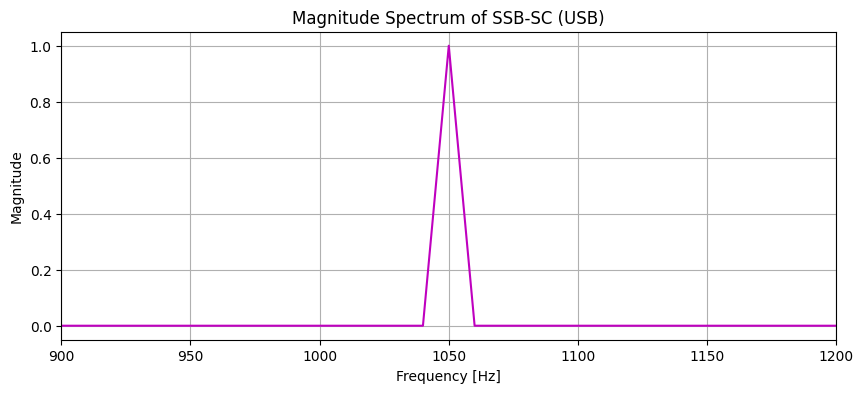
\includegraphics[width=0.9\textwidth]{images/output9.png} 
    \caption{Frequency-domain plot of the SSB-SC signal (USB)}
    \label{fig:phase_output2}
\end{figure}

\begin{figure}[H]
    \centering
    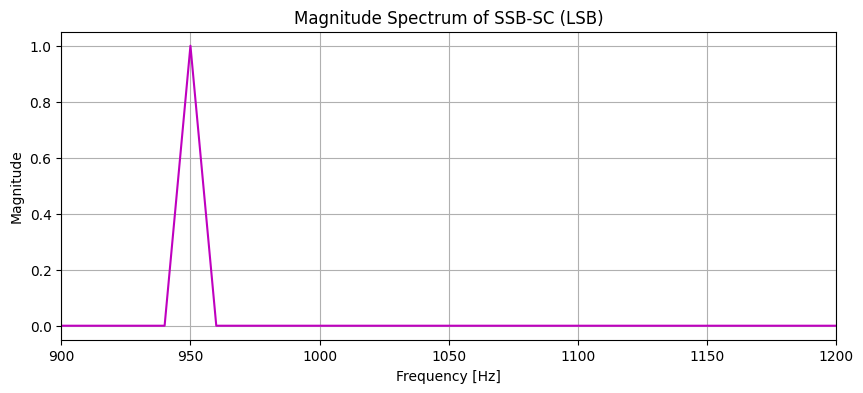
\includegraphics[width=0.9\textwidth]{images/output10.png} 
    \caption{Frequency-domain plot of the SSB-SC signal (LSB)}
    \label{fig:phase_comparison}
\end{figure}


\subsubsection*{Observations:}
In the Phase Discrimination method for SSB-SC signal generation, the carrier is completely suppressed and only the desired sideband (either upper or lower) is retained. Unlike the Bandpass Filter (FDM) method, the sideband selection here does not depend on filter slope or order, resulting in a cleaner and more precise isolation of the single sideband. In the frequency domain, the spectrum shows a single peak corresponding to the selected sideband, demonstrating efficient bandwidth usage. 

Compared to the FDM method, which can suffer from incomplete suppression of the unwanted sideband when low-order filters are used, the phase discrimination method consistently provides a clean output.